\documentclass[12pt,fleqn]{article}\usepackage{../../common}
\begin{document}
Sezonsallık, Trend Çıkartmak, Değişim Noktası, CUSUM

Zaman serilerini trendini, sezonsallığını nasıl inceleriz, ve trendde değişim
varsa bunu nasıl yakalarız?

Bir örnek üzerinde görelim, bir şirketin şampuan satış kazancı, veri [1]'den,

\begin{minted}[fontsize=\footnotesize]{python}
import pandas as pd
def parser(x):
    return pd.datetime.strptime( '190'+x, '%Y-%m' )
    
df = pd.read_csv('shampoo-sales.csv', header=0, index_col=0, \
     parse_dates=True, date_parser=parser)
df.Satis.plot()
plt.savefig('tser_022_de_07.png')
\end{minted}

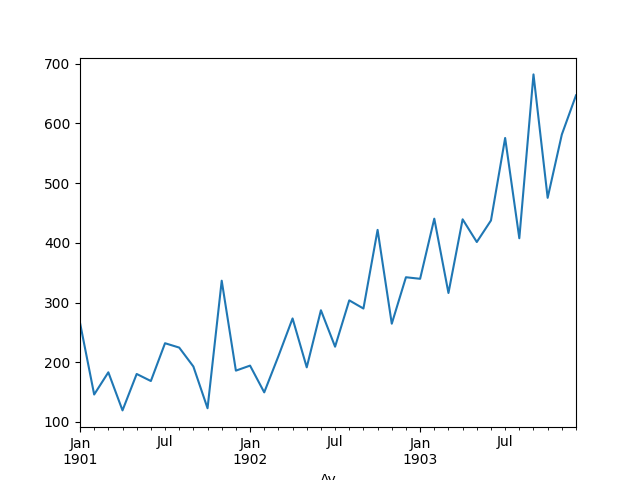
\includegraphics[height=6cm]{tser_022_de_07.png}

Yukarı doğru bir trend var. Bu trendi veriye bir düz çizgi uydurarak (fit), yani
tek değişkenli, ikinci derece lineer regresyon yaparak yakalayabiliriz. Bunu
yapmayı pek çok diğer derste gösterdik, \verb!statsmodels.regression!
paketinden, \verb!linear_model.OLS! ile, \verb!statsmodels.formula.api! ile,
ya da direk Lineer Cebir kullanarak.. Altta \verb!polyfit!  çağrısı
kullanılacak.

Modelden gelen katsayıları (coefficients) kullanıp tahmini $y$ değerleri üretmek
için alttaki fonksiyon var,

\begin{minted}[fontsize=\footnotesize]{python}
def model_compute(X, coef):
   degree = len(coef)-1
   curve = [np.sum([coef[-1]] + [x**(degree-d)*c for d,c \
            in enumerate(coef[:-1])]) for x in X]
   return curve
\end{minted}

Uydurmayı yapıp modeli veri üzerinde gösterelim,

\begin{minted}[fontsize=\footnotesize]{python}
X = np.array(range(len(df))).reshape(-1)
y = df.values.reshape(-1)
degree = 1
coef = np.polyfit(X, y, degree)
df['Model']  = model_compute(X, coef)
df.plot()
plt.savefig('tser_022_de_01.png')
\end{minted}

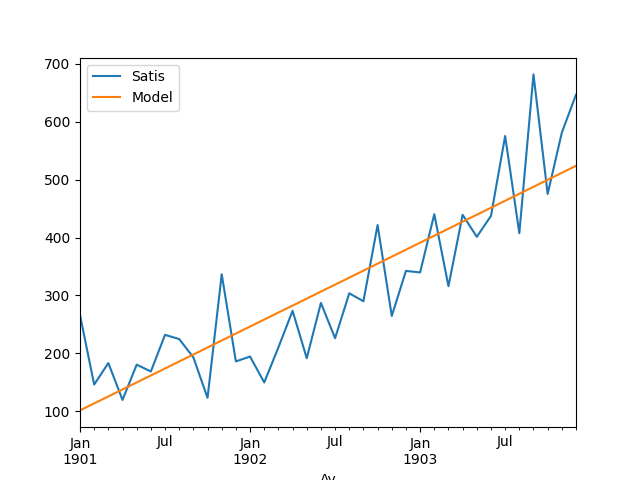
\includegraphics[height=6cm]{tser_022_de_01.png}

Veriden ``trendi çıkartabiliriz''. Bunu basit bir şekilde veriden modeli
eksilterek yapabiliriz. Bu durumda geriye kalan sadece trend haricinde olan
şeyler olacaktır. Trend çıkartmanın pek çok amacı olabilir, belki trend
haricinde olan kalıpları, eğer hala varsa, görmek istiyoruz, ya da modelin
artığına (residual) bakarak onun gürültü olup olmadığını anlamak
istiyoruz. Bilindiği gibi lineer regresyonun faraziyesi verinin model artı
gürültü olduğudur, o zaman model veriden çıkartılınca geriye kalan artık,
``tortu'' sadece gürültüdür. Gürültünün matematiksel tanımı Gaussian, ya da
Normal dağılımıdır, demek ki artıklar üzerinde normallik testi bir anlamda
modelin uyma başarısını da ölçer.

\begin{minted}[fontsize=\footnotesize]{python}
detrended = df.Satis-df.Model
detrended.plot()
plt.savefig('tser_022_de_03.png')
\end{minted}

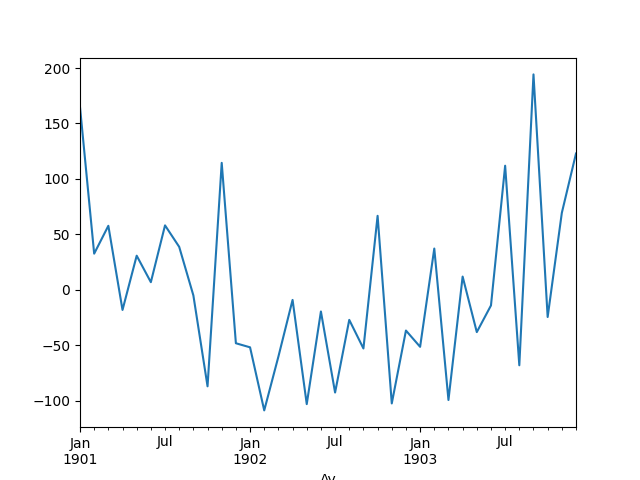
\includegraphics[height=6cm]{tser_022_de_03.png}

Normallik testini uygulayalım,

\begin{minted}[fontsize=\footnotesize]{python}
from scipy import stats
val,pval = stats.shapiro(detrended)
print ('p degeri =', pval)
\end{minted}

\begin{verbatim}
p degeri = 0.09782794862985611
\end{verbatim}

Shapiro-Wilk testinde p-değerinin 0.05'ten küçük olması normalliğin reddedilmesi
demektir. Üstte normal olmadığın reddedemedik, demek ki büyük ihtimalle elimizde
bir Normal dağılım var.

Sezonsallık

Benzer bir şekilde sezonşallığı da modelleyebiliriz. Sezonsallık bir
periyotsallığı ima eder, o zaman en genel şekilde bir sinüs fonksiyonunu veriye
uydurabiliriz. Fakat bu sinüs fonksiyonunun benliğini, başlangıç noktasını
bilmiyoruz, bu durumlarda [6]'da sinüssel regresyon tekniğini gördük. Fakat
belki de daha rahatı veriye bir 4'üncü derece polinom uydurmaktır.

Bu garip gelebilir, polinom uydurmayı çoğunlukla ikinci, üçüncü derecede
eğrileri modelleyen çerçevede görmüş olabiliriz, bu yaklaşım fakat periyotsal
fonksiyonları da çok rahat temsil edebiliyor. Sebebi herhalde sinüs fonsiyonunun
Taylor açılımında [3] gizli, Taylor açılımında sonsuza kadar giden türevler
polinom açılımda kullanılır, sinüsün 1'den 4'e kadar olan türevlerine bakarsak,

$\sin^{\prime}(x)=\cos(x),\quad$
$\sin^{\prime\prime}(x)=-\sin(x),\quad$,
$\sin^{\prime\prime\prime}(x)=-\cos(x),\quad$,
$\sin^{(4)}(x)=\sin(x)$.

Dördüncü türevin tekrar $\sin(x)$'a dönüş yaptığını görüyoruz. Demek ki 4'üncü
derece polinom açılımı periyotsal fonksiyonları temsil etmek için yeterlidir.

Altta bir bölgeden alınmmış günlük, o günün minimum hava sıcaklığı ölçümlerini
görüyoruz. Ona modeli uyduralım,

\begin{minted}[fontsize=\footnotesize]{python}
import pandas as pd
df = pd.read_csv('daily-min-temperatures.csv', header=0,\
                 index_col=0, parse_dates=True)
X = [i%365 for i in range(0, len(df))]
y = df.values
degree = 4
coef = np.polyfit(X, y, degree)
df['Model']  = model_compute(X, coef)
df.plot()
plt.savefig('tser_022_de_02.png')
\end{minted}

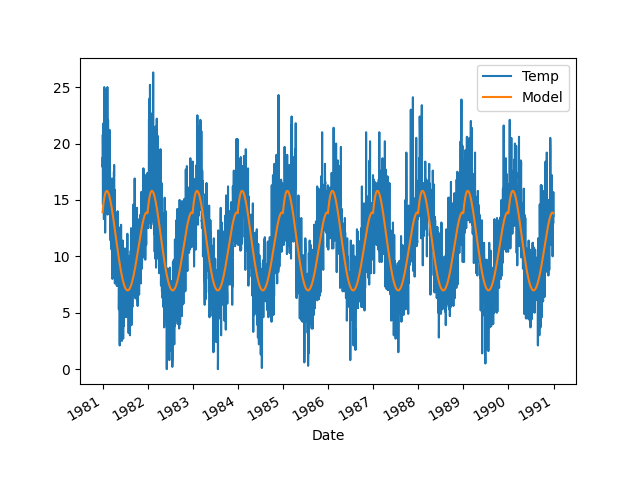
\includegraphics[height=6cm]{tser_022_de_02.png}

Periyotsallık yakalanmış gibi duruyor. Sezonsallığı veriden çıkartalım,

\begin{minted}[fontsize=\footnotesize]{python}
deseasoned = df.Temp-df.Model
deseasoned.plot()
plt.savefig('tser_022_de_04.png')
\end{minted}

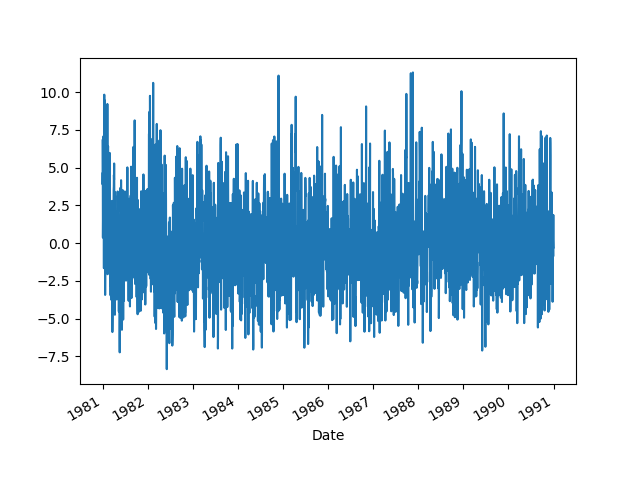
\includegraphics[height=6cm]{tser_022_de_04.png}

Artıklar üzerinde normallik testi,

\begin{minted}[fontsize=\footnotesize]{python}
from scipy import stats
val,pval = stats.shapiro(deseasoned)
print ('p degeri =', pval)
\end{minted}

\begin{verbatim}
p degeri = 4.155807920014354e-10
\end{verbatim}

Normal değil. Bunun sebebi veri içinde birden fazla sezonsallık, ya da başka bir
örüntünün hala mevcut olması olabilir. Bu senaryoları test etmek ödev olsun.

Yapısal Kopuş (Structural Break) Uygulaması

Üstteki teknikleri zaman serisinde ``ciddi'' bir değişim olup olmadığı, varsa
nerede olduğunun bulmak için kullanmak mümkündür. Yapısal kopuş için Chow
testini [7]'de ve Poisson bazlı [8]'de görmüştük.

Üstteki teknikleri kullanarak bir yaklaşım herhangi bir nokta öncesi ve sonrası
zaman serisi parçalarını almak, ve önceki parçada lineer regresyon, yapıp
katsayıları alıp gürültünün normalliğini kontrol etmektir. Eğer normallik varsa,
katsayılar alınıp ikinci parçada kullanılır, gürültü yine normalse kopuş yoktur
(aynı zaman serisi). Birincide gürültü normalliği yoksa kopuş yine yoktur, ilk
parça doğru tanımlı değil. Sezonsallık benzer şekilde kontrol edilebilir, vs.

Cusum

Cusum yaklaşımı [5] makalesinde araştırılmış, özyineli (recursive), yani teker
teker her yeni veri noktası üzerinde işlem yapan ve kopuşları o anda yakalamaya
uğraşan bir yaklaşımdır. Özyineli regresyon konusunu [4]'te gördük. Bir
regresyon hipotezi ile başlayıp her veri noktası geldiğinde regresyonu
güncellemek, iyileştirmek mümkündür. Cusum bunu yapar aynı anda modelin
gürültüsünü kontrol eder ve zaman serisinin bazı hipotezlere uyup uymadığını her
defasında kontrol eder, uyum yoksa kopuş yakalanmış demektir.

Faraziye şudur, normal kopuksuz bir zaman serisi her anda $\beta_t$ vektöründe
katsayılara sahipse, modelden geri kalan gürültünün ortalaması (mean) sıfır
olacaktır, ve her anda $\sigma_t$ varyasyonu için,

$$
\beta_1 = \beta_2 = ... = \beta_T = \beta
$$

$$
\sigma_1^2 = \sigma_2^2 = ... = \sigma_T^2 = \sigma
$$

Yani her anda katsayılar ve gürültünün varyasyonu sabit olmalı. Cusum
$\beta_t$'deki değişimi yakalamak için ayarlanmıştır, bunu yapmak için gürültü
ortalamasının sıfırdan sapmasını yakalamaya uğraşır. Detayları için Cusum
makalesine danışılabilir.

Alttaki kod [2]'yi temel alıyor. 

\inputminted[fontsize=\footnotesize]{python}{cusum.py}

Örnek bir zaman serisinde görelim,

\begin{minted}[fontsize=\footnotesize]{python}
import pandas as pd
  
y = np.random.randn(300)/5
y[100:200] += np.arange(0, 4, 4/100)
x = range(len(y))
df = pd.DataFrame(y,columns=['y'])
df['x'] = x
df = df.set_index('x')
df.y.plot()
plt.savefig('tser_022_de_05.png')
\end{minted}

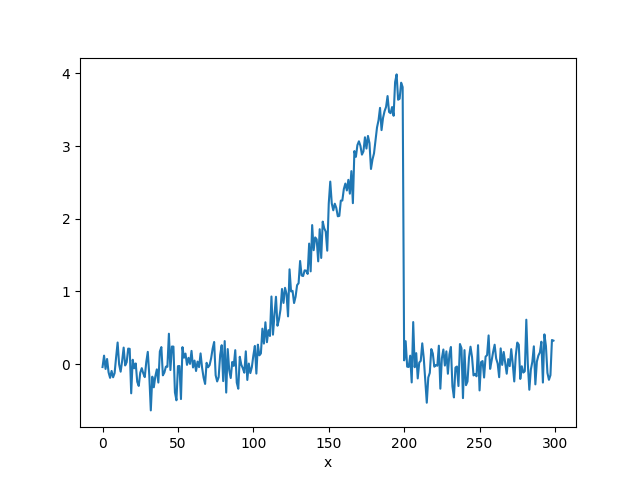
\includegraphics[height=6cm]{tser_022_de_05.png}

Bu zaman serisinde bariz kopuşlar var, yaklaşık indeks 100 anında, sonra
200 anında. Cusum ile bunları yakalamaya uğraşalım,

\begin{minted}[fontsize=\footnotesize]{python}
import cusum
ta, tai, taf, amp = cusum.detect_cusum(df.y, 2, .02, True, True)

print (len(ta))
print ('Baslangic =', tai[0], 'Bitis =', taf[0])
\end{minted}

\begin{verbatim}
2
Baslangic = 95 Bitis = 197
\end{verbatim}

Geri döndürülen \verb!tai!, \verb!taf! birer vektördür, ve sırasıyla kopuş
noktasının başlangıç ve bitiş indisini verirler. Yukarıda ilk kopuşun
indisini görüyoruz.

Grafiklersek,

\begin{minted}[fontsize=\footnotesize]{python}
fig, ax = plt.subplots(1, 1)
t = range(df.y.size)
ax.plot(t, df.y, 'b-', lw=2)
if len(ta):
    ax.plot(tai, df.y[tai], '>', mfc='g', mec='g', ms=10, label='Start')
    ax.plot(taf, df.y[taf], '<', mfc='g', mec='g', ms=10, label='Ending')
    ax.plot(ta, df.y[ta], 'o', mfc='r', mec='r', mew=1, ms=5, label='Alarm')
    
plt.savefig('tser_022_de_06.png')
\end{minted}

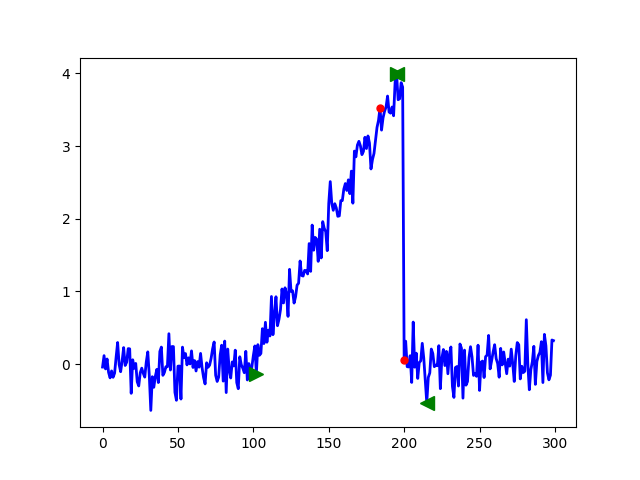
\includegraphics[height=6cm]{tser_022_de_06.png}

Sağa dönük yeşil ok başlangıç, sola dönük bitiş demek. En tepede ikisi
birbirinin üstüne bindi çünkü orada bir parça bitip diğeri başlıyor, ama olanlar
gözüküyor herhalde. Kırmızı noktalar ise alarm anları olarak tanımlanmış. 

Kaynaklar

[1] Brownlee, {\em Introduction to Time Series Modeling with Python}

[2] Github, \url{https://raw.githubusercontent.com/BMClab/BMC/master/functions/detect_cusum.py}

[3] MIT, {\em OCW Single Variable Calculus, unit 5, Session 99},
         \url{https://ocw.mit.edu/courses/mathematics/18-01sc-single-variable-calculus-fall-2010/index.htm}

[4] Bayramli, {\em Hesapsal Bilim, Ders 1-15}
         
[5] Brown, et al, {\em Techniques for Testing the Constancy of Regression Relationships over Time}

[6] Bayramli, {\em Zaman Serileri, Sinüssel Regresyon (Sinusoidal Regression)}

[7] Bayramli, {\em Istatistik, Testlere devam}

[8] Bayramli, {\em Istatistik, Değişim Noktası Analizi}

\end{document}
